\documentclass[ngerman]{dtk}
\usepackage[utf8]{inputenc}
\usepackage[]{hyperref}
\usepackage[]{babel}
\usepackage[]{csquotes}
\usepackage[]{listings}
\usepackage[]{paralist}
\usepackage[]{xcolor,xspace}

\definecolor{hellgelb}{rgb}{1,1,0.8}
\definecolor{colKeys}{rgb}{0,0,0.6}
\definecolor{colIdentifier}{rgb}{0,0,0}
\definecolor{colComments}{rgb}{1,0,0}
\definecolor{colString}{rgb}{0,0.5,0}
\definecolor{darkblue}{rgb}{0,0,0.6}

\lstset{literate=%
    {Ö}{{\"O}}1
    {Ä}{{\"A}}1
    {Ü}{{\"U}}1
    {ß}{{\ss}}1
    {ü}{{\"u}}1
    {ä}{{\"a}}1
    {ö}{{\"o}}1
    {~}{{\textasciitilde}}1
}

\newcommand{\ep}{euro\textit{pass}\xspace}

\title{\ep Lebensläufe setzen mit \LaTeX} 
\Author{Uwe}{Ziegenhagen}{Köln} 

\begin{document}
\maketitle
\markboth{euro\textit{pass}}{euro\textit{pass}}

\begin{abstract}
In diesem Artikel sollen mit \texttt{ecv} und \texttt{europecv} zwei Pakete vorgestellt werden, die den Satz von Lebensläufen nach dem europäischen euro\textit{pass} Muster ermöglichen.
\end{abstract} 

\section{Der Europäische Lebenslauf}

Die \ep Initiative der Europäischen Union hat das Ziel, ein Rahmenwerk für grenzüberschreitende Bewerbungsunterlagen zu schaffen. 

Innerhalb eines Landes lassen sich verschiedene Bewerbungen noch relativ einfach vergleichen, bei Bewerbungen aus verschiedenen europäischen Ländern wird dies jedoch schwer, da es in den einzelnen Ländern unterschiedliche Bewertungsmaßstäbe gibt.

Mit \ep ist ein Standard geschaffen worden, der Qualifikationen, Fähigkeiten und Kompetenzen europaweit verständlich darstellen will. Ein komplettes Qualifikationsprofil besteht dabei aus den folgenden Dokumenten:

\begin{compactitem}
\item euro\textbf{\textit{pass}} Lebenslauf
\item euro\textbf{\textit{pass}} Sprachenpass
\item euro\textbf{\textit{pass}} Mobilität
\item euro\textbf{\textit{pass}} Diploma Supplement
\item euro\textbf{\textit{pass}} Zeugniserläuterungen
\end{compactitem}


\section{Das \texttt{ecv} Paket}

Das \texttt{ecv} Paket von Chr.~Neumann und B.~Haberstumpf bietet eine eigene eigene Dokumentenklasse, die in ihrer aktuellen Form deutsch und englisch als globale Optionen (\texttt{[german]} bzw. \texttt{[english]}) unterstützt. Beide Sprachen lassen sich in einem Dokument nutzen, die entsprechenden \texttt{ecv}-Befehle unterstützen alle optionale Argumente für die Angabe der Sprache. In seiner aktuellen Version 0.3 vom April 2011 setzt das Paket \texttt{latin9} Encoding voraus, dies lässt sich jedoch durch einfaches Austauschen gegen beispielsweise \texttt{utf8} in der \texttt{ecv.cls} beheben.

Für zentrale Angaben wie den in der Fußzeile genutzten Namen oder die Angabe des Bewerbungsfotos stellt das Paket die folgenden Befehle bereit:

\begin{compactitem}
\item \verb|\ecvPortrait{Datei}| setzt das Bewerbungsfoto
\item \verb|\ecvName{Vorname Nachname}| setzt den Namen in der Fußzeile
\item \verb|\ecvSig{Name}{Ort}| setzt die Unterschrift
\end{compactitem}

\subsection{Definition der Überschriften}

Die einzelnen Lebensabschnitte werden dann innerhalb einer \texttt{ecv}-Umgebung gesetzt. Um einen Lebenslauf zu unterteilen, gibt es eine Reihe von Kommandos:

\begin{compactitem}
\item \verb|\ecvSec[lang]{Text}| Section-Befehl 
\item \verb|\ecvBSec[lang]{Text}| Section-Befehl mit vertikalem Abstand
\item \verb|\ecvSub[lang]{Text}| Subsection-Befehl 
\item \verb|\ecvBSub[lang]{Text}| Subsection-Befehl mit vertikalem Abstand
\item \verb|\ecvERSub[lang]{Text}{Text}| Subsection-Befehl mit rechtsbündiger Beschreibung
\item \verb|\ecvBERSub[lang]{Text}{Text}| Subsection-Befehl mit rechtsbündiger Beschreibung und Abstand 
\item \verb|\ecvEBSub[lang]{Text}{Text}| Subsection-Befehl mit Beschreibung im Blocksatz
\item \verb|\ecvBEBSub[lang]{Text}{Text}| Subsection-Befehl mit Beschreibung im Blocksatz und Abstand 
\end{compactitem}

Verschiedene Befehle stehen für lokalisierte Strings bereit, die je nach Spracheinstellung (\texttt{[german]} bzw. \texttt{[english]}) den deutschen bzw. englischen Begriff  setzen:

\begin{compactitem}
\item \verb|\ecvPerson| für \enquote{Person} bzw.  \enquote{Personal Information}
\item \verb|\ecvProfession| für \enquote{Beruf} bzw.    \enquote{Profession}
\item \verb|\ecvResearch| für \enquote{Forschung} bzw.   \enquote{Research}
\item \verb|\ecvEducation| für \enquote{Ausbildung} bzw.    \enquote{Education}
\item \verb|\ecvPublications| für \enquote{Publikationen} bzw.   \enquote{Publications}
\item \verb|\ecvAwards| für \enquote{Auszeichnungen} bzw.   \enquote{Awards}
\item \verb|\ecvScholarships| für \enquote{Stipendien} bzw.    \enquote{Scholarships}
\item \verb|\ecvJobs| für \enquote{Berufserfahrung} bzw.   \enquote{Jobs}
\item \verb|\ecvLanguages| für \enquote{Sprachen} bzw.   \enquote{Languages}
\item \verb|\ecvLanguageTravels| für \enquote{Sprachreisen} bzw.   \enquote{Language Travels}
\item \verb|\ecvAbilities| für \enquote{Fähigkeiten} bzw.   \enquote{Abilities}
\item \verb|\ecvConferences| für \enquote{Konferenzen} bzw.   \enquote{Conferences}
\item \verb|\ecvSpeeches| für \enquote{Vorträge} bzw.   \enquote{Speeches}
\item \verb|\ecvTraining| für \enquote{Fortbildungen} bzw.    \enquote{Training}
\item \verb|\ecvAttachements| für \enquote{Anhänge} bzw.    \enquote{Attachements}
\end{compactitem}

Für die einzelnen Einträge innerhalb eines Abschnitts gibt es ebenfalls verschiedene Befehle, die gleichzeitig \enquote{Tag} und \enquote{Text} setzen, dabei entspricht \enquote{Tag} der auf der linken Seite stehenden Bezeichnung des Eintrags, \enquote{Text} der rechtsseitig stehenden Beschreibung selbst: 

\begin{itemize}
\item \verb|\ecvEPR[lang]{Tag}{Text}| setzt ein einfaches Tag, rechtsbündig
\item \verb|\ecvEPB[lang]{Tag}{Text}| setzt ein einfaches Tag im Blocksatz
\item \verb|\ecvEFR[lang]{Tag}{Text}| setzt ein  rechtsbündiges Bullet-Tag
\item \verb|\ecvEFB[lang]{Tag}{Text}| setzt ein Bullet-Tag im Blocksatz
\item \verb|\ecvENR[lang]{Tag}{Text}| setzt einen rechtsbündigen Eintrag 
\item \verb|\ecvENB[lang]{Tag}{Text}| setzt einen Eintrag im Blocksatz
\end{itemize}

Es gibt auch die Möglichkeit, \enquote{Tag} und \enquote{Text} getrennt zu setzen, hier sei auf die Anleitung des Pakets \cite{ecv} verwiesen. In Listing \ref{l1} ist ein komplettes Beispiel abgedruckt:

\begin{lstlisting}[language={[LaTeX]TeX},caption={Beispiel für das \texttt{ecv} Paket},basicstyle=\ttfamily\footnotesize,identifierstyle=\color{colIdentifier},keywordstyle=\color{colKeys},%
inputencoding={utf8},extendedchars=true,backgroundcolor=\color{hellgelb},stringstyle=\color{colString},commentstyle=\color{colComments}, label={l1}]
\documentclass[german]{ecv}
\usepackage[T1]{fontenc}
\usepackage{babel}
\ecvPortrait{../Bilder/Mustermann.png}
\begin{document}
\begin{ecv}
\ecvSec{\ecvPerson}
\ecvEPR{Name}{Erika Mustermann}
\ecvEPR[german]{Adresse}{Beethovenallee~37a\newline 146612~Berlin}
\ecvEPR[english]{Address}{Beethovenallee~37a\newline 146612~Berlin}
\ecvEPR[german]{Telefon}{(030)6912415}
\ecvEPR[english]{Phone}{+49306912415}
\ecvEPR{E-Mail}{erika.mustermann@gmx.net}
\ecvEPR[german]{Staatsangehörigkeit}{Deutsch}
\ecvEPR[english]{Nationality}{German}
\ecvEPR[german]{Geburtsdatum}{13.~September~1964}
\ecvEPR[english]{Birthdate}{September 13th 1964}
\ecvBSec{\ecvEducation}
\ecvBSub[german]{Schule}
\ecvBSub[english]{School}
\ecvEPR[german]{08/1971--05/1983}{Grundschule und Gymnasium 
in Berlin (Leistungskurse Mathematik und Physik)}
\ecvEPR[english]{08/1971--05/1983}{Elementary school and grammar school
in Berlin (major fields mathematics and physics)}
\end{ecv}
\ecvSig{Erika Mustermann}{Berlin}
\end{document}
\end{lstlisting}


\begin{figure}
\centering
\fbox{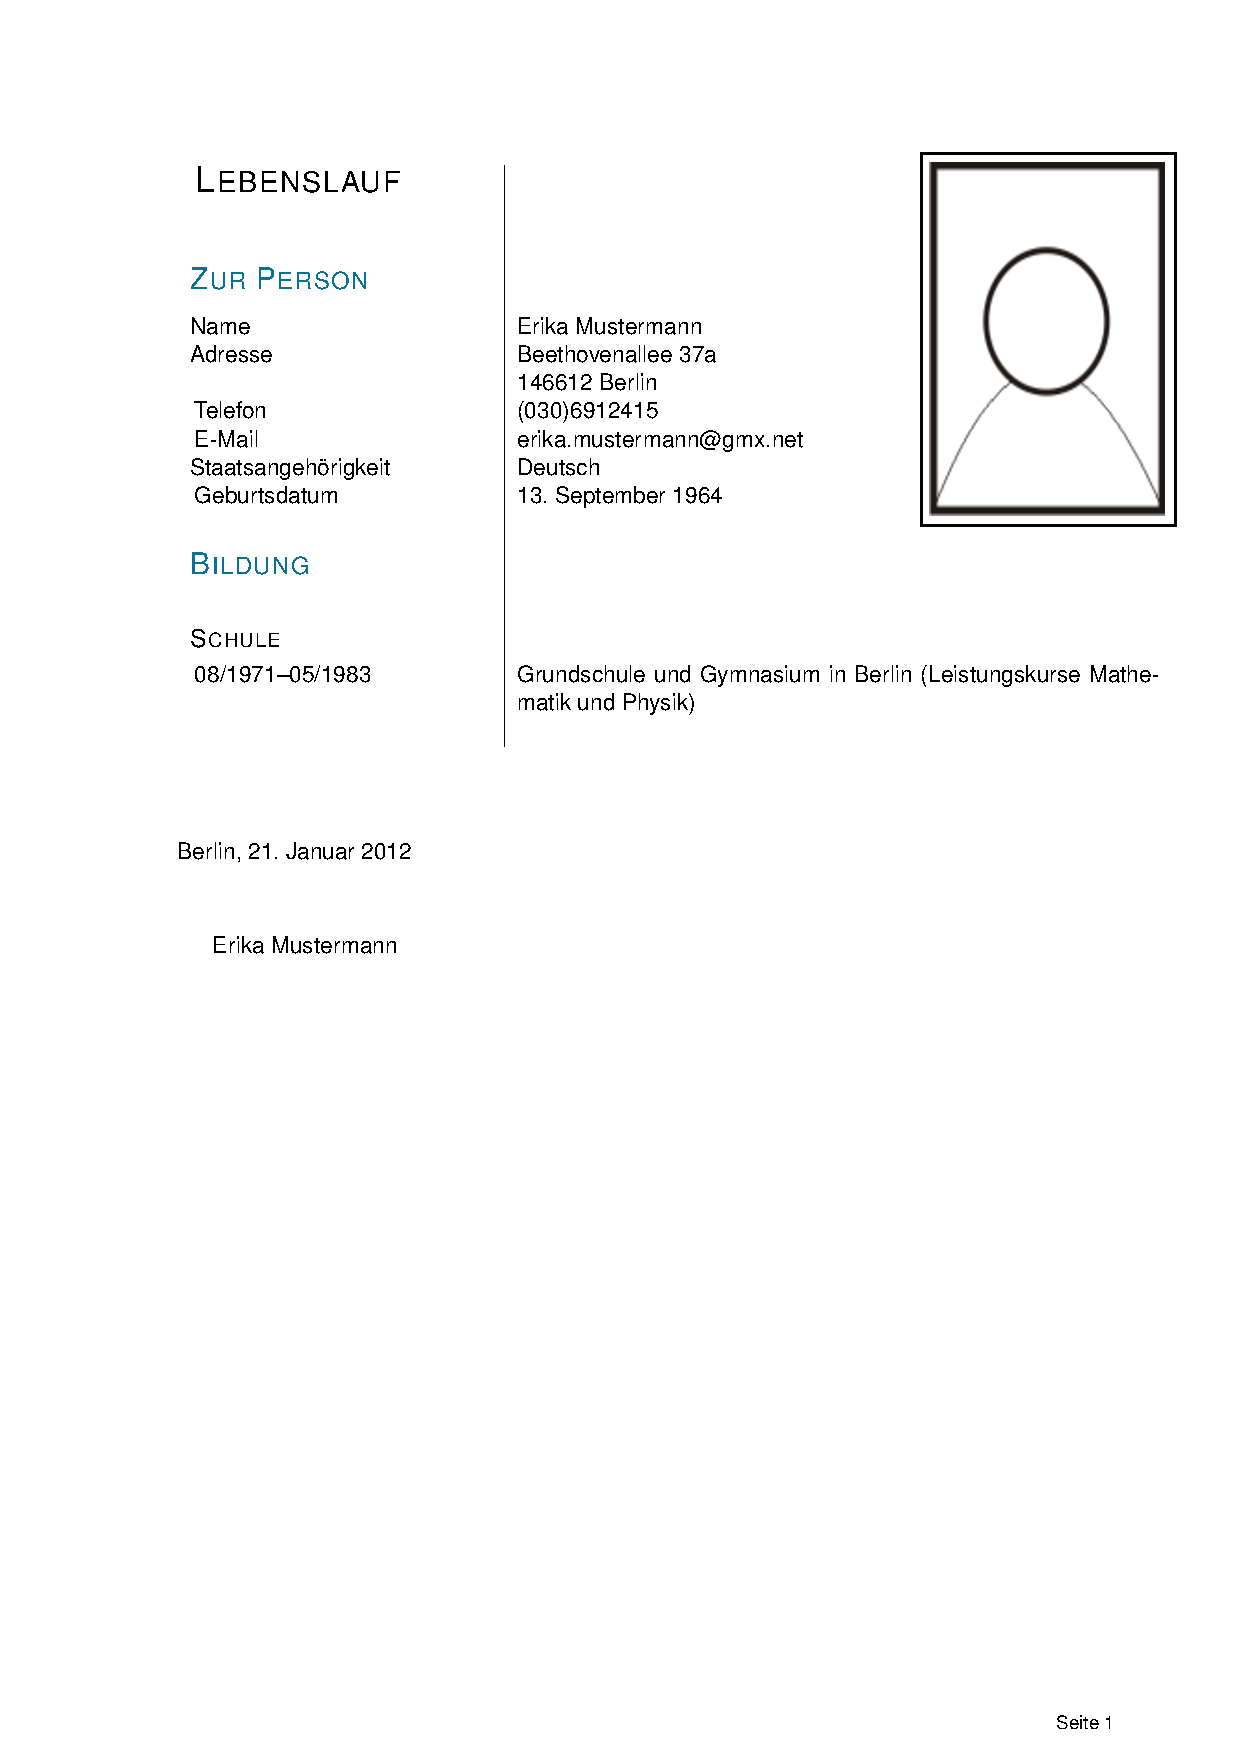
\includegraphics[width=0.9\textwidth]{ecv/ecvtest.pdf}}
\caption{Ausgabe von Listing \ref{l1}, deutsches \texttt{ecv} Beispiel}
\end{figure}


\section{Das \texttt{europecv} Paket}

Im Gegensatz zu \texttt{ecv} unterstützt das \texttt{europecv} Paket von Nicola Vitacolonna aus dem Jahr 2006 quasi alle europäischen Sprachen, isländisch und maltesisch dürften hierbei sicherlich die exotischsten Vertreter sein.

Wie \texttt{ecv} stellt \texttt{europecv} eine eigene Klasse bereit, der andere Pakete wie \texttt{totpages} oder  \texttt{booktabs} per Klassenoption übergeben werden können. Der Lebenslauf selbst wird dann in einer \texttt{europecv} Umgebung gesetzt. 

Für die Angabe von persönlichen Daten wie Name, Adresse und Telefonnummer bietet \texttt{europecv} eine Reihe von Befehlen, die automatisch in die in der Klassenoption angegebenen Sprache übersetzt werden.

\begin{compactitem}
\item \verb|\ecvname{Text}| setzt den Namen
\item \verb|\ecvfootername{Text}| setzt den Namen in der Fußzeile 
\item \verb|\ecvaddress{Text}| setzt die Adresse 
\item \verb|\ecvtelephone[mobil]{Telnr}| setzt die Telefonnummer
\item \verb|\ecvfax{Faxnummer}|  setzt die Faxnummer
\item \verb|\ecvemail{Text}|  setzt  die E-Mail Adresse
\item \verb|\ecvnationality{Text}| setzt die Angabe der Nationalität
\item \verb|\ecvdateofbirth{Datum}| setzt das Geburtsdatum
\item \verb|\ecvgender{Text}| setzt die Angabe des Geschlechts
\item \verb|\ecvpicture{Bild}| setzt das Bewerbungsfoto
\end{compactitem}

Sind die entsprechenden Angaben definiert, lassen sie sich durch \verb|\ecvpersonalinfo| setzen. Für die Gruppierung und den Satz der einzelnen Elemente des Lebenslaufs stellt \texttt{europecv} zwei Befehle bereit: 

\begin{itemize}
 \item \verb|\ecvsection[vspace]{Text}| Abschnittsname mit optionalem vertikalen Abstand
 \item \verb|\ecvitem[vspace]{Tag}{Beschreibung}| Eintrag mit Tag und Beschreibung und optionalem vertikalen Abstand
\end{itemize}

\subsection{Sprachkenntnisse}

Die Beschreibung der Sprachkenntnisse eines Bewerbers ist in \texttt{europecv} besonders umfassend gelöst; Hier implementiert das Paket die Vorgabe von \ep.

\ep unterteilt die Beherrschung einer Fremdsprache in fünf Kategorien: verstehendes Hören (l1), verstehendes Lesen (l2), kommunikatives Sprechen (l3), erzählendes Sprechen (l4) und Schreiben (l5). 

Die Kenntnisse jeder dieser Kategorien soll jeder Bewerber von A1 bis C2 bewerten, für Details zu den einzelnen Niveaus siehe die Anleitung des Pakets \cite{europecv} oder den entsprechenden Wikipedia-Artikel \cite{rahmen}. 

\begin{compactitem}
\item \verb|\ecvAOne| basic user (A1)
\item \verb|\ecvATwo| basic user (A2)
\item \verb|\ecvBOne| independent user (B1)
\item \verb|\ecvBTwo| independent user (B2)
\item \verb|\ecvCOne| proficient user (C1)
\item \verb|\ecvCTwo| proficient user (C2)
\end{compactitem}

Die Sprachbefähigung wird dann in Form einer Tabelle ausgegeben. Die folgenden Befehle setzen die einzelnen Teile der Tabelle.

\begin{compactitem}
 \item \verb|\ecvmothertongue[vspace]{Sprache}| setzt die Muttersprache
 \item \verb|\ecvlanguageheader[vspace]{Symbol}|  setzt den Kopf der Sprachtabelle mit Referenz auf die CEF-Fußnote, \texttt{Symbol} definiert das Fußnotensymbol
 \item \verb|\ecvlanguagefooter[vspace]{Symbol}|  druckt die CEF-Zeile, \texttt{Symbol} definiert das Fußnotensymbol 
 \item \verb|\ecvlanguage[vspace]{Sprache}{l1}{l2}{l3}{l4}{l5}|  setzt eine Zeile der Tabelle
 \item \verb|\ecvlastlanguage[vspace]{Sprache}{l1}{l2}{l3}{l4}| setzt dann die letzte Zeile, wenn \texttt{booktabs} per Klassenoption geladen wurde
\end{compactitem}

\begin{figure}[h]
\centering
\fbox{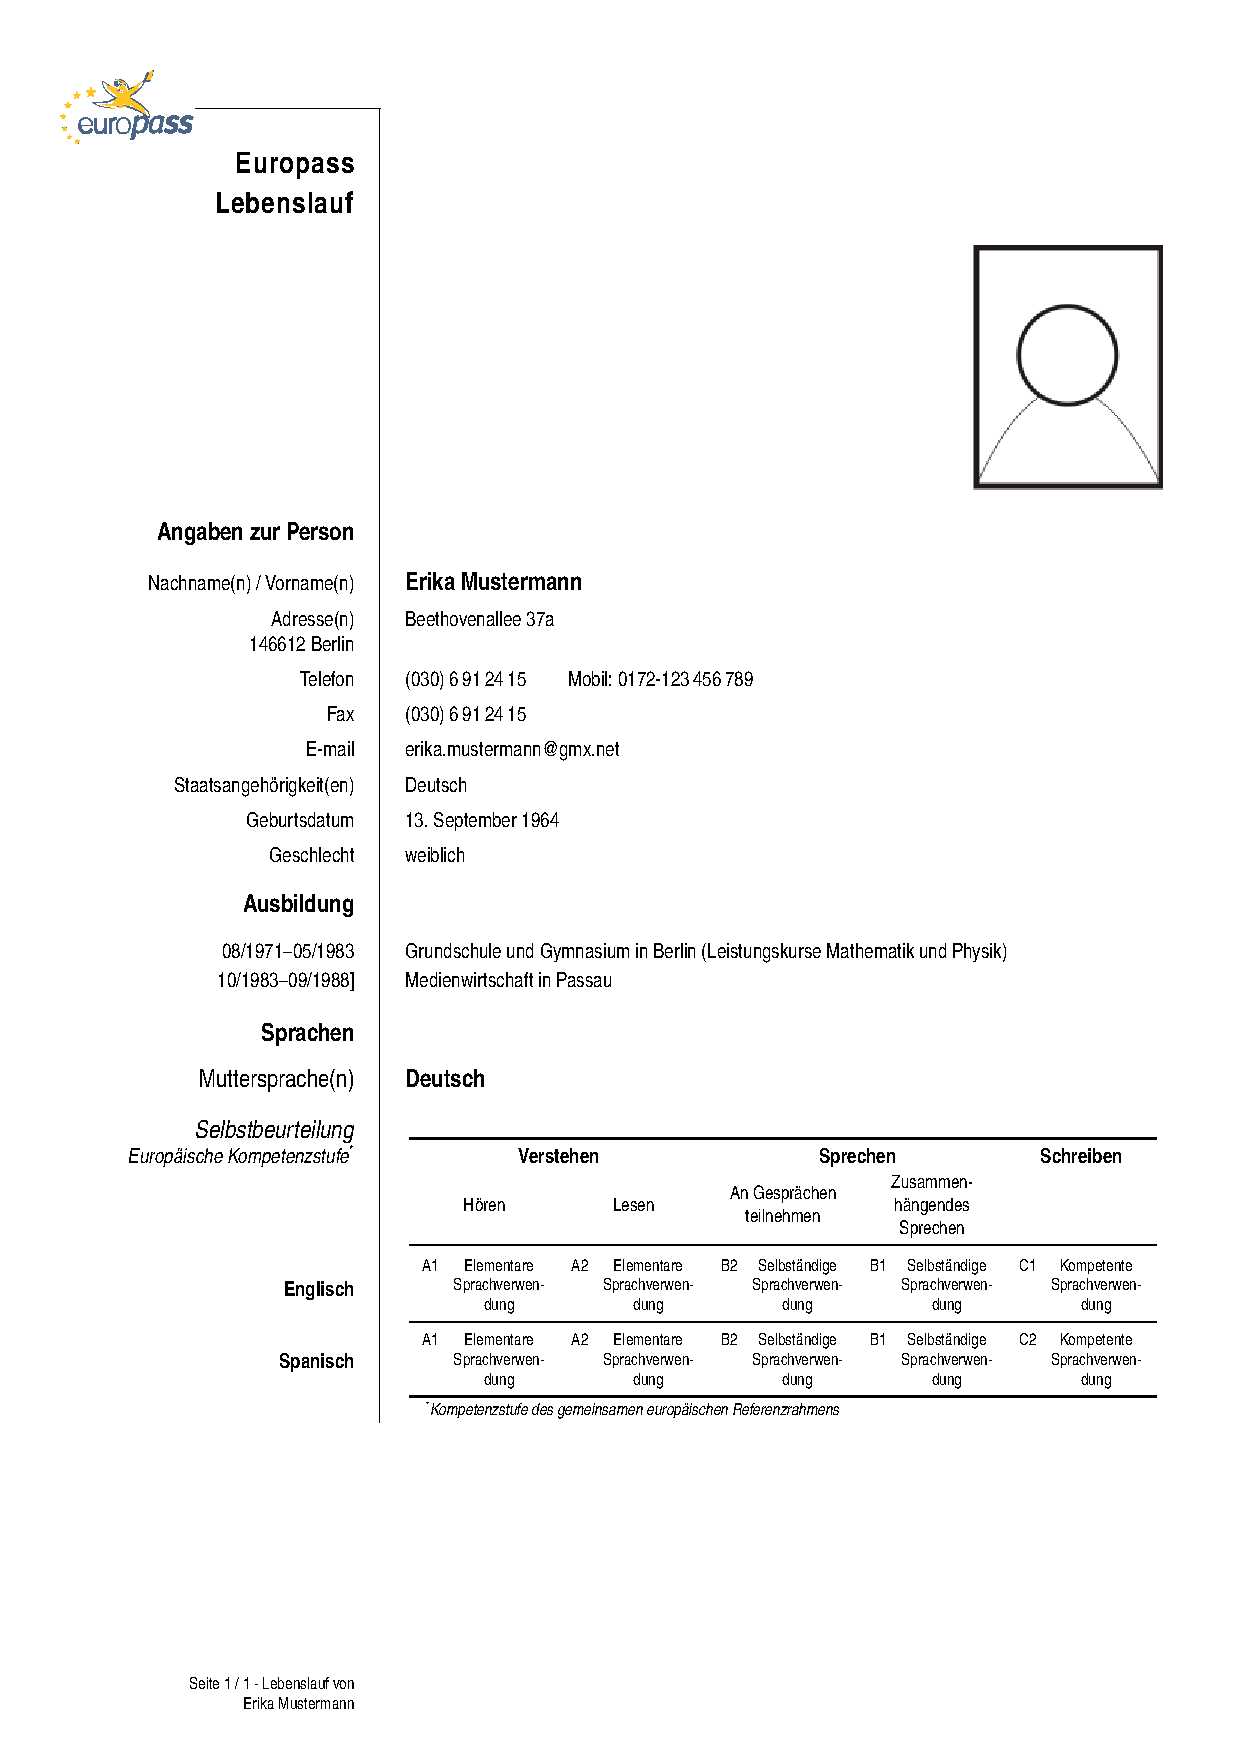
\includegraphics[width=0.9\textwidth]{europecv/europecvtest.pdf}}
\caption{Ausgabe von Listing \ref{l2}, europecv}\label{fig:europecv}
\end{figure}

\begin{lstlisting}[language={[LaTeX]TeX},caption={Beispiel für das \texttt{europecv} Paket, siehe Abbildung \ref{fig:europecv} auf Seite \pageref{fig:europecv}},basicstyle=\ttfamily\footnotesize,identifierstyle=\color{colIdentifier},keywordstyle=\color{colKeys},backgroundcolor=\color{hellgelb},stringstyle=\color{colString},commentstyle=\color{colComments}, label={l2}]
\documentclass[a4paper,helvetica,narrow,german,latin1,totpages, booktabs]{europecv}
\usepackage[a4paper,top=1.5cm,left=1cm,right=1.3cm,bottom=2.0cm]{geometry}
\usepackage[T1]{fontenc}
\usepackage{babel}
\usepackage[]{graphicx}

\ecvname{Erika Mustermann} 
\ecvfootername{Erika Mustermann} 
\ecvaddress{Beethovenallee~37a\\ 146612~Berlin}
\ecvtelephone[0172-123\,456\,789]{(030)~6\,91\,24\,15}
\ecvfax{(030)~6\,91\,24\,15}
\ecvemail{erika.mustermann@gmx.net}
\ecvnationality{Deutsch}
\ecvdateofbirth{13. September 1964}
\ecvgender{weiblich}
\ecvpicture{../Bilder/Mustermann.png}

\begin{document}
\begin{europecv}
\ecvpersonalinfo

\ecvsection{Ausbildung}
\ecvitem{08/1971--05/1983}{Grundschule und Gymnasium in Berlin 
(Leistungskurse Mathematik und Physik)}
\ecvitem{10/1983--09/1988]}{Medienwirtschaft in Passau}

\ecvsection{Sprachen}
\ecvmothertongue[12pt]{Deutsch}
\ecvlanguageheader{*}
\ecvlanguage{Englisch}{\ecvAOne}{\ecvATwo}{\ecvBTwo}{\ecvBOne}{\ecvCOne}
\ecvlastlanguage{Spanisch}{\ecvAOne}{\ecvATwo}{\ecvBTwo}{\ecvBOne}{\ecvCTwo}
\ecvlanguagefooter{*}
\end{europecv}
\end{document}
\end{lstlisting}


\section{Fazit}

Beide Pakete bieten sehr interessante Möglichkeiten, einen professionell aussehenden Lebenslauf nach EU-Standard zu setzen. Welches Paket man am Ende vorzieht, sollte man anhand eines kleinen Musterdokuments selbst entscheiden. Anhand des Funktionsumfangs der beiden Pakete lässt sich keine klare Empfehlung für das eine und gegen das andere aussprechen. Das \texttt{ecv}-Paket punktet beim Satz von deutscher und englischer Version des Lebenslaufs, \texttt{europecv} ist im Umgang etwas einfacher und bietet eine sehr ansprechende Darstellung der Sprachkompetenz. 
 
Die Beispieldateien zu diesem Artikel liegen unter \url{http://www.uweziegenhagen.de/?p=1333}. Für Kommentare und Anregungen bin ich jederzeit dankbar.

\end{document}